\documentclass[10pt]{article}
%\usepackage{anysize}
%\papersize{11in}{8.5in}
%\marginsize{1in}{1in}{.5in}{.5in}
\textwidth = 6.5 in
\textheight = 9 in
\oddsidemargin = 0.0 in
\evensidemargin = 0.0 in
\topmargin = -0.5 in
\headheight = 0.35 in
\headsep = 0.15 in
\topskip = 0 in
\footskip = 0.5 in
\pagenumbering{arabic}
\usepackage{setspace}
\usepackage[usenames]{color}
\usepackage[fleqn]{amsmath}
\usepackage{graphicx}
\usepackage{url}
\usepackage{verbatim}
\usepackage{indentfirst}
\usepackage{booktabs}
\usepackage{multirow}
\usepackage[table]{xcolor}
\usepackage{ragged2e}
\usepackage{xspace}
\usepackage{parskip}
\usepackage{tabulary}
\usepackage[normalem]{ulem}
\usepackage{hyperref}
\hypersetup{pdfborder={0 0 0}, colorlinks=true, urlcolor=blue, linkcolor=black}
\usepackage[format=plain, labelsep=period, justification=raggedright, singlelinecheck=true, skip=2pt, font={footnotesize,sf}, labelfont=bf]{caption}
\usepackage{titlesec}
\usepackage{lastpage}
\usepackage{fancyhdr}
\usepackage{ifthen}
\usepackage{wrapfig}
\usepackage{cleveref}
\crefformat{footnote}{#2\footnotemark[#1]#3}

%\usepackage[round]{natbib}
%\bibliographystyle{evolution}
% \usepackage[style=nature]{biblatex}
\usepackage[bibstyle=bib/joaks-statement,maxcitenames=3,mincitenames=2,backend=biber]{biblatex}

\newrobustcmd*{\shortfullcite}{\AtNextCite{\renewbibmacro{title}{}\renewbibmacro{in:}{}\renewbibmacro{number}{}}\fullcite}

\bibliography{references}

%% Format headers and footers %%%%%%%%%%%%%%%%%%%%
\pagestyle{fancy}
%\lhead{\ifthenelse{\value{page}=1}{}{\sffamily\footnotesize Jamie Oaks}}
\lhead{\sffamily \emph{\docTitle} \\ Jamie R. Oaks}
%\chead{\ifthenelse{\value{page}=1}{{\scshape \docTitle} \\ Jamie Richard Oaks}{\sffamily\footnotesize \docTitle}}
%\rhead{\ifthenelse{\value{page}=1}{}{\sffamily\footnotesize \today}}
\rhead{\sffamily \today}
\cfoot{\sffamily\footnotesize Page \thepage\ of \pageref{LastPage}}
\renewcommand{\headrulewidth}{0.4pt}
\renewcommand{\footrulewidth}{0pt}

%% Format section titles %%%%%%%%%%%%%%%%%%%%%%%%%
\renewcommand\refname{Peer-reviewed Publications}

\titleformat{\section}[hang]
    {\large\sffamily\bfseries}
    {\S\ \thesection.}{.5em}{}[]
\titlespacing{\section}
    {0mm}{1.0ex plus .1ex minus .1ex}{-0.5ex}

\titleformat{\subsection}[hang]
    {\large\sffamily\itshape}
    {\S\ \thesection.}{.5em}{}[]
\titlespacing{\subsection}
    {0mm}{1.0ex plus .1ex minus .1ex}{-0.5ex}

\titleformat{\subsubsection}[runin]
    {\sffamily\bfseries}
    {\S\ \thesection.}{.5em}{}[.---]
\titlespacing{\subsubsection}
    {\parindent}{0pt}{0pt}
%    {\parindent}{1.0ex plus .1ex minus .1ex}{0pt}

%% Format list environments %%%%%%%%%%%%%%%%%%%%%%%%
\renewcommand{\labelenumii}{\arabic{enumi}.\arabic{enumii}}
\renewcommand{\labelitemi}{$\circ$}

\newenvironment{myEnumerate}{
  \begin{enumerate}
    \setlength{\itemsep}{0.25em}
    \setlength{\parskip}{0pt}
    \setlength{\parsep}{0.5em}}
  {\end{enumerate}}

\newenvironment{myItemize}{
  \begin{itemize}
    \setlength{\leftskip}{-4mm}
    \setlength{\itemsep}{0.25em}
    \setlength{\parskip}{0pt}
    \setlength{\parsep}{0.5em}}
  {\end{itemize}}

%% Basic formatting and spacing %%%%%%%%%%%%%%%%%%%%%
\setlength{\parindent}{0em}
\setlength{\parskip}{0.5em}

%% My functions %%%%%%%%%%%%%%%%%%%%%%%%%%%%%
\newcommand{\ignore}[1]{}
\newcommand{\addTail}[1]{\textit{#1}.---}
\newcommand{\super}[1]{\ensuremath{^{\textrm{#1}}}}
\newcommand{\sub}[1]{\ensuremath{_{\textrm{#1}}}}
\newcommand{\dC}{\ensuremath{^\circ{\textrm{C}}}}
\newcommand{\tableSubItem}{\addtolength{\leftskip}{1em} \labelitemi \xspace}
\newcommand{\myHangIndent}{\hangindent=5mm}

%%%%%%%%%%%%%%%%%%%%%%%%%%%%%%%%%%%%%%%%%%%%%%%%%%%%%%%%%%%%%%
%%%%%%%%%%%%%%%%%%%%%%%%%%%%%%%%%%%%%%%%%%%%%%%%%%%%%%%%%%%%%%
\newcommand{\docTitle}{Research Statement\xspace}
\begin{document}
% \raggedright
\singlespacing

% \textbf{\textit{What processes shape genetic variation both temporally and
%         spatially, partition evolutionary lineages, and generate and maintain
%         biodiversity?}} \\
\textbf{\textit{What processes control the generation and assembly of
        biodiversity?}}
Elucidating answers to this question is the primary motivation of my research
program.
To address this question, I use patterns of genetic variation within and among
species to identify independent evolutionary lineages (i.e., species) and infer
their demographic histories and relationships, testing for patterns predicted
by current ecological factors and historical events.
I use a broad suite of methods in this endeavor, including
% collection-based fieldwork,
fieldwork,
collecting genome-wide DNA sequence data via next-generation sequencing (NGS)
technologies,
developing model-based statistical procedures for inferring evolutionary
history from genomic datasets,
implementing such methods in software packages,
and ultimately applying these novel computational tools to genomic data to test
hypotheses about diversification.
% I take an integrative approach to answering open-ended questions about
% biodiversity, which requires critical thinking and creativity.
% As a result, it is imperative that I involve students with diverse
% backgrounds and interests, who can bring unique perspectives to the
% challenges in my lab.
Given the integrative nature of my research program, I seek to recruit students
with diverse backgrounds and interests.
The questions I am passionate about exploring are open-ended and require
critical thinking and creativity.
As a result, it is imperative that I involve students and collaborators with
diverse backgrounds and perspectives to bring together unique insights.

\section*{Previous Research}
%%%%%%%%%%%%%%%%%%%%%
% \subsection*{Diversification of Crocodiles}
% Traditionally, crocodiles (\emph{Crocodylus}) have been stereotyped as an
% ancient group of ``living fossils'' that originated in Africa prior to the
% fragmentation of Pangea; their diversity and circumtropical distribution was
% attributed to vicariance via continental drift.
% However, early molecular data and subsequent reassessment of paleontological
% data suggested the genus could be younger than previously believed.
% Recently, I collected a large multi-locus dataset of all extant crocodylian
% species and used novel statistical phylogenetic methods to infer the temporal
% and biogeographical origin of \emph{Crocodylus}.
% My results overturned traditional views of crocodiles as ``living-fossils''
% from Africa, revealing a recent and dynamic evolutionary history
% \footfullcite{Oaks2011}.
% My results strongly support that all extant crocodiles shared a common ancestor
% from the tropics of the Indo-Pacific, approximately 14--8 million years ago
% (mya), rejecting an ancient vicariant explanation of their biogeography in
% favor of a recent, dispersal-mediated model involving multiple transoceanic
% dispersals.
% It was not until after the mid-Miocene climatic optimum, when the global
% climate was cooling and fellow crocodylian lineages were suffering massive
% extinctions, that \emph{Crocodylus} radiated and dispersed around the globe.
% This finding suggests it was not only global cooling driving the extinction of
% other crocodylians, as previously believed, but also most likely competition
% with the rapidly radiating \emph{Crocodylus} lineage.
% %My results also revealed more species diversity within the \emph{Crocodylus}
% %than currently recognized.

% This study also introduced important methodological innovations.
% To accommodate the variation of substitution rates across DNA positions
% within and among genes, I used a novel approach of estimating the optimal model
% for partitioning the alignment into rate categories.
% The resulting model performed far better than traditional methods that
% partition the alignment based on \emph{a priori} expectations of rate variation
% \footfullcite{OaksInPrep}.
% This has important implications, because improved modeling of among-site rate
% variation will mitigate the underestimation of long branches and concomitant
% systematic error in phylogenetic estimates (e.g., long-branch attraction).
% Furthermore, the study was among the first to estimate a time-calibrated
% species tree using a multi-species coalescent model, and was the first to use a
% posterior sample of species trees to estimate ancestral-state reconstructions.
% % The species tree represents the evolutionary history of populations, rather
% % than the history of individual gene copies.
% Using a direct estimate of the species phylogeny, rather than the history of
% individual gene copies, is ideal when inferring the evolutionary patterns of
% species-level characters, like ancestral ranges.

\subsection*{Climate-driven diversification}
One question I am passionate about is whether Quaternary climatic oscillations
promoted diversification by fragmenting the distributions of species.
% One focus of my current research seeks to determine whether Quaternary climatic
% oscillations promoted diversification by fragmenting the distributions of
% species.
An ideal model system for addressing this question is the dynamic landscape of
Southeast Asia.
The Southeast Asian mainland and complex system of 26,000+ islands experienced
dramatic cyclical shifts in the extent of the terrestrial landscape during
Quaternary glacial cycles.
Many groups of islands in this region coalesced into aggregate islands during
glacial periods when sea levels were up to 120m below current level; these
islands were repeatedly fragmented during interglacial rises in sea level.

% \begin{wrapfigure}{r}{0.44\textwidth}
%   \vspace{-1.5em}
%   \begin{center}
%       \fbox{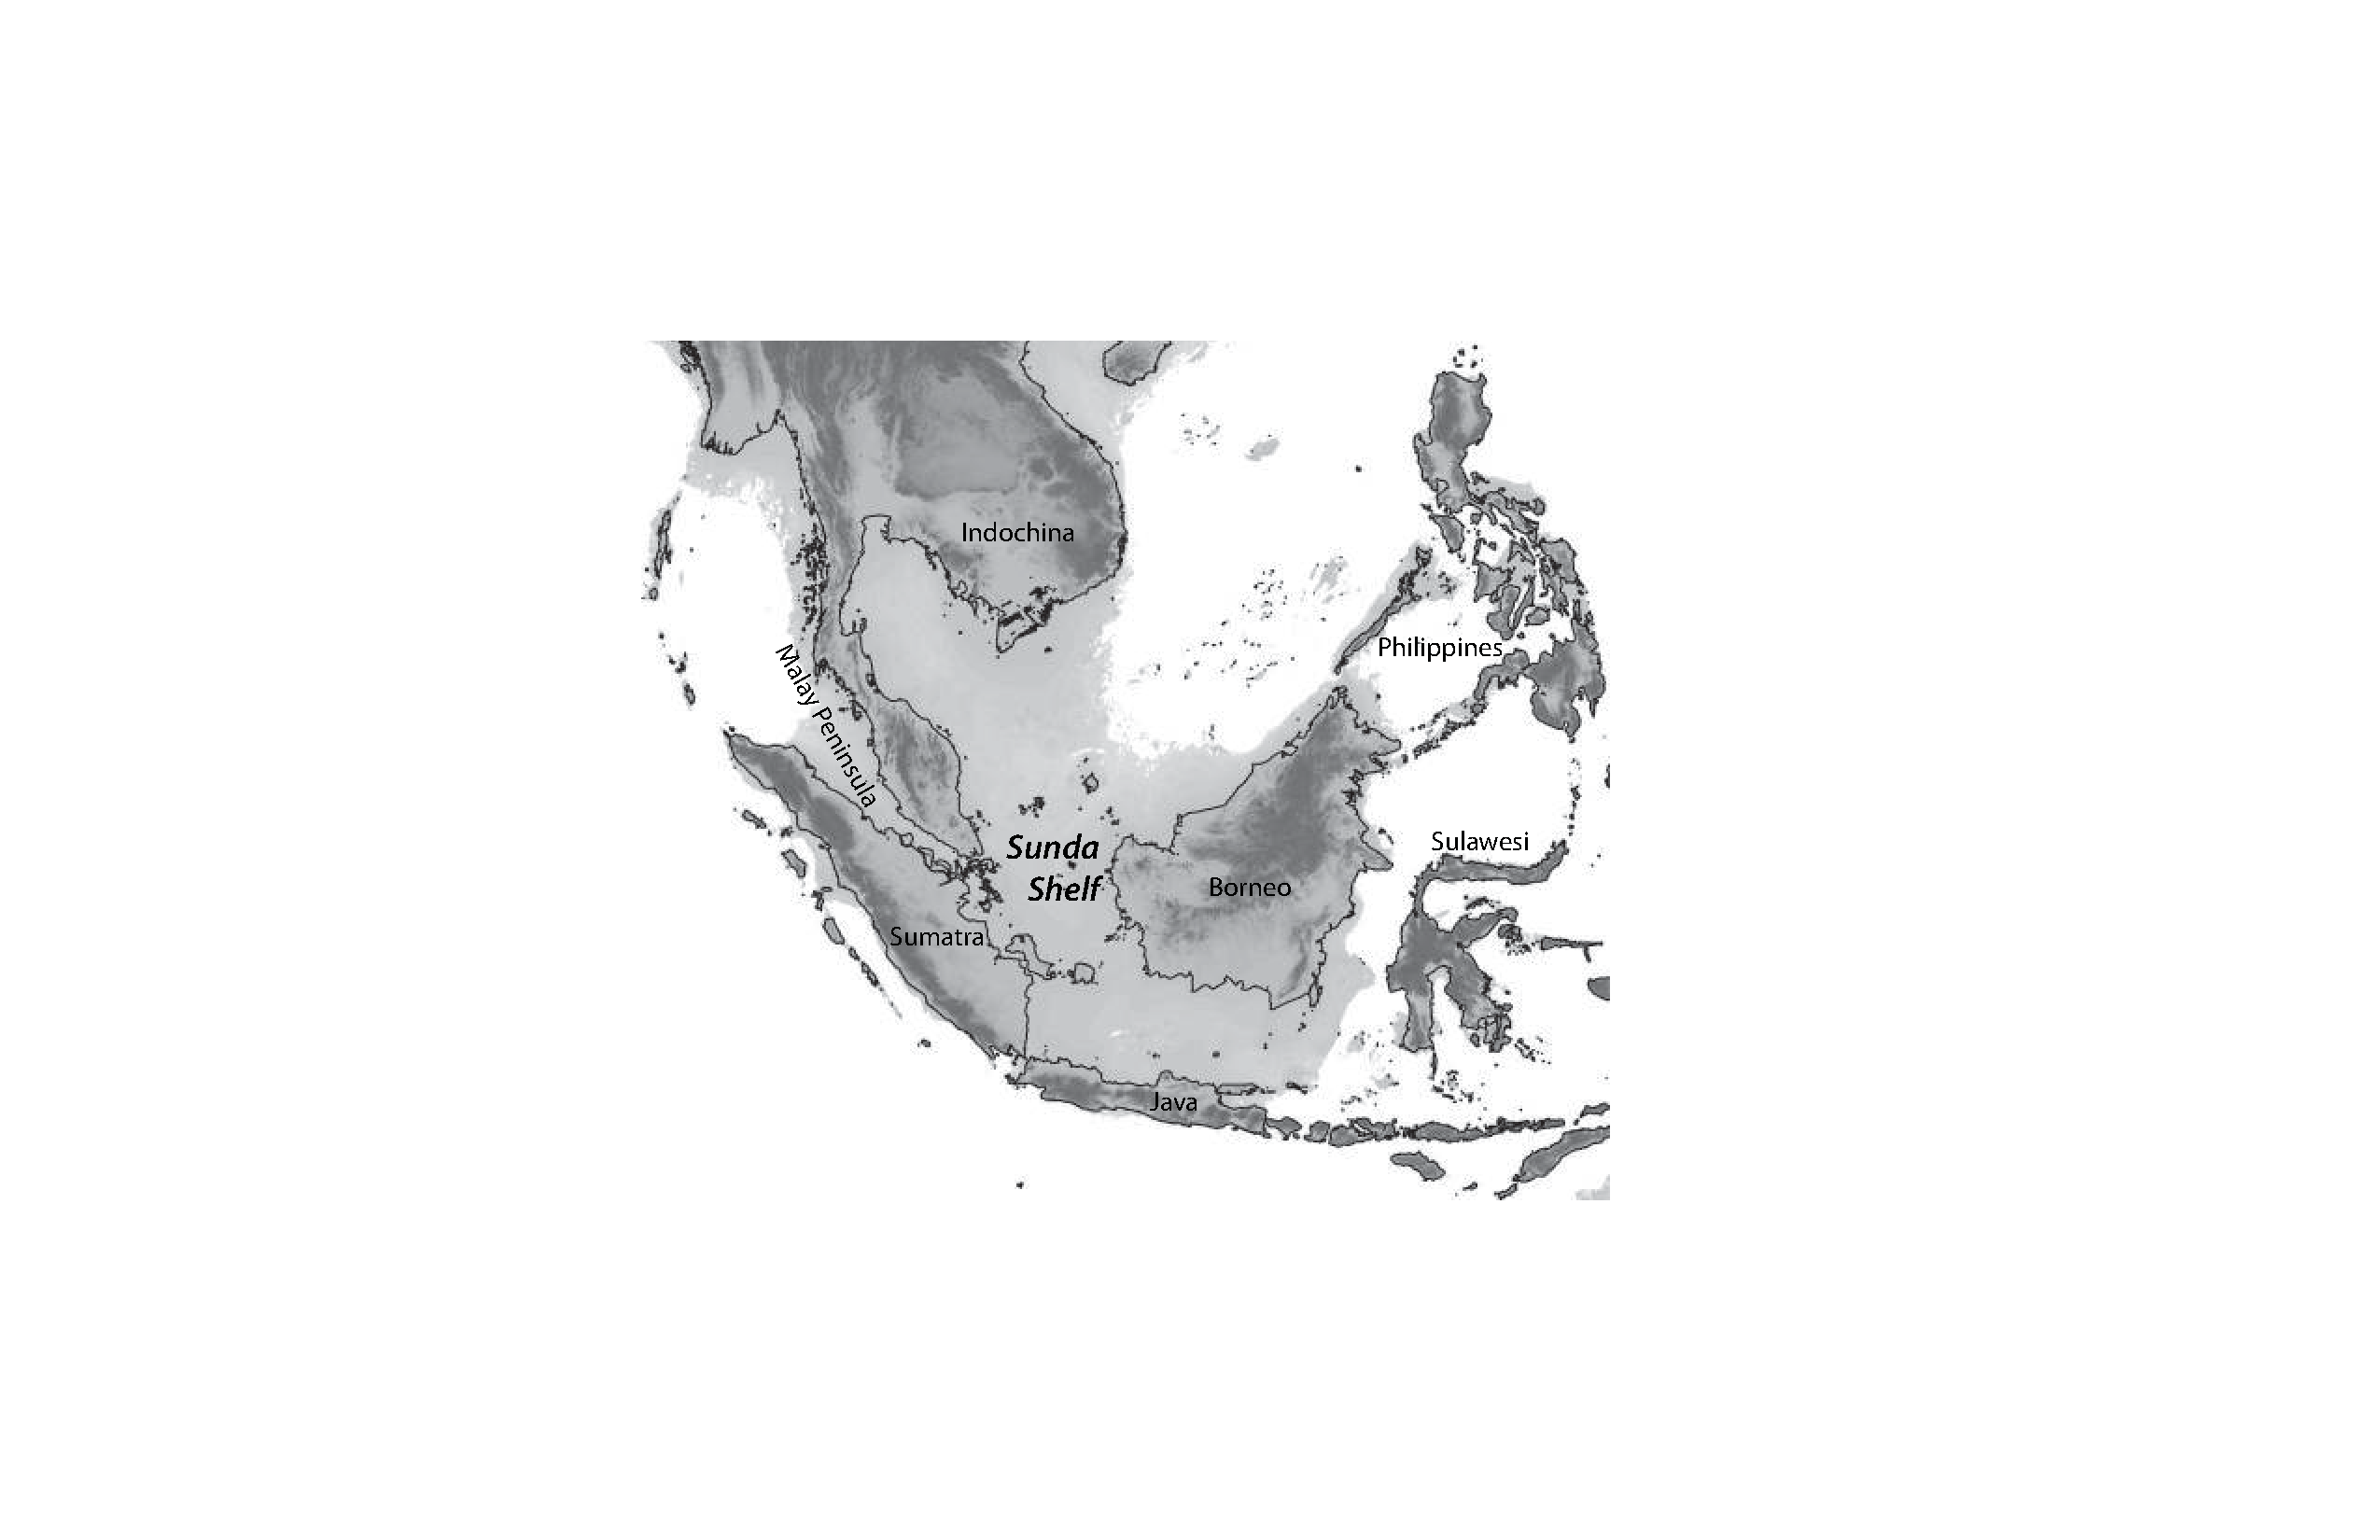
\includegraphics[width=0.43\textwidth]{sunda_shelf_very_small.pdf}}
%   \end{center}
%   \vspace{-0.2em}
%   \caption{Map of Southeast Asia with land extent (depicted in grey) during
%   glacial lowstands estimated using 120m bathymetry (data from
%   \href{http://ngdc.noaa.gov/mgg/global/global.html}{ETOPO1}).}
%   \label{map}
%   \vspace{-1.1em}
% \end{wrapfigure}

To test whether the repeated formation and fragmentation of island complexes
promoted diversification, collaborators and I have been studying the
evolutionary history of two genera of geckos (\emph{Cyrtodactylus} and
\emph{Gekko}) that are co-distributed across most of the islands of the
Philippines\footnote{\label{Siler10}\shortfullcite{Siler2010}}\super{,}\footnote{\label{Siler12}\shortfullcite{Siler2012}}.
We found that populations within island complexes did explain a significant
proportion of the genetic diversity, but were not monophyletic, and there was
no obvious pattern of diversification associated with Pleistocene glacial
cycles.
We revealed complex histories for both genera that contradict many of the
traditional areas of endemism predicted by island connectivity during glacial
periods.
Interestingly, for \emph{Gekko}, we found evidence that the genus colonized the
Philippines by ``rafting'' on the Palawan Microcontinental Islands that rifted
away from Mainland Asia and drifted toward the rest of the Philippine
Archipelago.

In order to more directly test whether glacial cycles promoted
diversification, we used a broadly comparative approach\cref{Oaks12}.
We accumulated genetic data from island populations of 22 distantly related
taxa, representing five orders of terrestrial vertebrates.
For each taxon, we sampled genetic data from two populations currently on
separate Philippine Islands that were previously connected during glacial
periods.
If repeated bouts of island connectivity and isolation promoted
diversification, the temporal distribution of divergences across the 22
inter-island pairs of populations should be temporally clustered and correspond
to interglacial rises in sea level that fragmented the islands.
To test this prediction, we employed a popular Bayesian model-choice method,
msBayes, to estimate the probabilities of models in which multiple sets of taxa
diverged at the same time.
We found very strong support
% (posterior probability of 0.982)
for a single, recent, simultaneous divergence event shared by all 22 taxa.

Suspicious of such strong support given the richness and stochasticity of the
candidate models,
I used computer simulations to assess the ability of the msBayes method to
detect random variation in divergence times.
The results of the simulations revealed that the method will often strongly
support highly clustered models of divergence even when the taxa being compared
diverged randomly over millions of generations.
Thus, our results from the empirical Philippines data were likely spurious.
% This finding is important, because msBayes is a popular method, and results of
% clustered divergence times across co-distributed taxa are often interpreted as
% evidence for a shared historical event.
% Our results demonstrate that the method can be biased toward such results, and
% the interpretation of a shared event is not warranted without simulation-based
% validation of the method's performance.

% Needed better method---did it
Rather than abandon the approach, I formulated the full evolutionary model
underlying the simulation-based msBayes procedure and, using first 
principles of probability, identified theoretical reasons the method
would tend to spuriously infer simultaneous divergence across
taxa\footnote{\label{Oaks12}\shortfullcite{Oaks2012}}\super{,}\footnote{\label{Oaks14reply}\shortfullcite{Oaks2014reply}}.
Guided by these insights, I developed a new model that uses more flexible prior
probability distributions for many of the models' parameters, and a
nonparametric Dirichlet-process prior across all possible divergence models.
I implemented the new model in the software package dpp-msbayes, and developed
a much more efficient multi-processing interface for both dpp-msbayes and
msBayes.
Using analyses of simulated and empirical data, I found, as predicted by
theory, the new method was much more accurate and robust\cref{Oaks14dpp}.
Applying this new method to the comparative Philippines dataset, I found a
large amount of uncertainty about the number of divergence events shared across
the 22 taxa; there simply was not enough information in our data to
discriminate among models of divergence.
While this result is more trustworthy and intuitive than what we found
with the original method, it was empirically unsatisfying.
Thus, my current work focuses on developing more powerful methods that can
leverage large, comparative NGS datasets for addressing questions about
diversification.


\section*{Current Research}
%%%%%%%%%%%%%%%%%%%%%
Currently, I am developing and implementing novel statistical methods,
collecting comparative genomic datasets from biodiverse regions of the planet,
and applying the former to the latter to enable unprecedented power to
understand the historical processes of diversification across regions
characterized by high levels of species richness and endemism.
Below I detail one such method, and three empirical systems that have inspired
its development.

% Full likelihood method
\subsection*{Implementing a full-likelihood Bayesian comparative
    model of diversification}
While the method implemented in dpp-msbayes is more powerful and robust than
its predecessor, both methods are based on approximate likelihoods and discard
information when reducing the genetic data to a set of insufficient summary
statistics.
Thus, dpp-msbayes still struggles to discriminate among models of divergence at
recent evolutionary timescales \footnote{\label{Oaks14dpp}\shortfullcite{Oaks2014dpp}}.
Given that such a statistical tool is integral to the evolutionary questions
I seek to answer in my empirical research,
I am currently developing a method that employs a similar hierarchical model in
a full-likelihood Bayesian framework.
% I am utilizing recent developments that analytically integrate over gene trees
% for biallelic data\footnote{\label{Bryant12}\shortfullcite{Bryant2012}}.
% This will remove the gene trees from the numerical approximation machinery and
% allow efficient sampling of divergence models and population divergence times
% using full likelihoods and Markov chain Monte Carlo.
By analytically integrating over gene trees, the method will efficiently handle
genome-scale datasets.
By utilizing all of the information in the data, the method promises to be much
more powerful than its approximate-Bayesian counterparts, and will also be
applicable at deeper evolutionary timescales.
This new tool will allow evolutionary biologists to better leverage comparative
genetic data to assess the affects of regional and global biogeographical
processes on biodiversity.

% Apply new method to genomic data from Philippine geckonids
\subsection*{Applying novel statistical methods to understand diversification
    in Southeast Asia}
% (2) collecting genome-scale data from dense sampling of \emph{Cyrtodactylus}
% and \emph{Gekko} from across the Philippine Archipelago using next-generation
% sequencing technology.
In addition to developing a full-likelihood Bayesian framework for inferring
co-diversification, I have also collected genome-wide sequence data from nearly
300 \emph{Cyrtodactylus} and \emph{Gekko} individuals from across the
Philippine Archipelago using NGS technology.
The combination of the new method and NGS data will allow us to better assess
the affect of sea-level fluctuations on diversification across oceanic islands
of Southeast Asia.

To complement to this work on oceanic islands, I am also working with an
international team of collaborators to better understand diversification in
mainland Southeast Asia.
My collaborators include
Dr.\ Cameron Siler of the University of Oklahoma,
Dr.\ Lee Grismer of La Sierra University,
Dr.\ Norhayati Ahmad of the Universiti
Kebangsaan Malaysia (UKM),
Dr.\ Shahrul Anuar Mohd Sah of the Universiti Sains Malaysia (USM),
and
Dr.\ Anchalee Aowphol of Kasetsart University.
Through years of extensive fieldwork, we have collected a large comparative
dataset of reptiles and amphibians from across much of the Sunda Shelf.
Along with additional field collecting, we are currently collecting sequence
data from many of these taxa.
We will apply the methods I am developing to test long-standing hypotheses
about the affect of biogeographical transition zones on the diversification of
Sunda Shelf biota, including the Isthmus of Kras, and current and paleo-river
systems.
We plan to seek funding from the NSF Biodiversity Discovery and Analysis
Program for this project.

\subsection*{Diversification of the highly endemic fauna of the Gobi Desert}
The Gobi is the largest desert in Asia and is a mosaic of rocky mountain ranges
surrounded by basins of sand dunes.
% I am interested in better understanding the origins of the unique and highly
% endemic biodiversity of this region.
An international team of collaborators (Jesse Grismer and Dr.\ Rafe Brown of
the University of Kansas, Dr.\ Natalia Ananjeva of the Russian Academy of
Sciences, Dr.\ Xianguang Guo of the Chinese Institute of Biology, and Dr.\
Nyamsuren Batsaikhan of the National University of Mongolia) and I were awarded
a grant from the National Geographic Society to better document and understand
the history of the unique assemblage of reptiles that inhabit this region.
Our goal is to collect genomic data from a set of focal sand and rock-adapted
taxa and use the comparative methods I am developing to
(1) infer their evolutionary origins,
(2) test for patterns of shared evolutionary history, and
(3) identify key processes that led to the diverse and unique fauna of this
region.
% We will use the data and results from our current National Geographic award to
% apply for funding from the NSF Phylogenetic Systematics Program to extend this
% project.

% Unfunded collaborator on Adam and Matt's pending NSF proposal to apply method
% Africa
\subsection*{Application of novel methods to understand diversification
in West-Central African rainforests}
I am working with Drs.\ Adam Leach\'{e} and Matthew Fujita to apply the novel
statistical methods described above to comparative NGS datasets
to elucidate the historical processes of diversification and community assembly
across West-Central African rainforests.
We are particularly interested in determining how Pliocene and Pleistocene
aridification cycles and associated rainforest fragmentation influenced
diversification across the Afro-tropics.
% I am a collaborator on a pending NSF proposal to extend this work that was
% recently submitted by Drs. Leach\'{e} and Fujita.

% Apply new method to sunda shelf (Malaysia/Thailand)

\section*{Future Research}
%%%%%%%%%%%%%%%

\subsection*{Theoretical and computational advances in phylogenetics}
The projects below will result in computational tools that will benefit a broad
community of researchers conducting biogeographical analyses. I will seek
funding from the NSF Phylogenetic Systematics Program to secure funds for the
necessary computational resources to develop, test, and deploy these methods.

\subsubsection*{Extending co-diversification model choice to a fully
    phylogenetic framework}
While the full-likelihood Bayesian method I am currently developing promises to
greatly improve the accuracy and power of inferring shared evolutionary
history, I have plans to go even further and integrate the approach into a
fully phylogenetic framework.
I will do this by implementing a novel hierarchical Bayesian model for
co-estimating the number and timing of divergence events across a phylogeny,
and the assignment of the internal nodes in the tree to the events, while
integrating over uncertainty in phylogeny, gene trees, and demographic and
mutational parameters.
Key advantages of this approach include the ability to
(1) estimate and accommodate variation in relative rates of mutation and
population sizes across the phylogeny while jointly estimating the divergence
history, and
(2) infer more complicated divergence histories than is possible with methods
restricted to comparing pairs of populations.
% The resulting method will provide a fully Bayesian statistical framework
% for determining whether the temporal pattern of divergences across taxa are
% consistent with predictions of historical processes.

\subsubsection*{Simultaneous estimation of population history and structure: A
novel approach}
Currently, the estimation of coalescent-based phylogenies of recently
diversified species entails a two-step process.
First, some variant of a genetic clustering algorithm is used to estimate how
many populations (or species) are represented in their sample, and assign
individuals to those populations.
Second, the relationships among the resulting clusters is then inferred under a
multi-species coalescent model.
This assumes the population assignment is estimated without error, which is
especially worrying because genetic clustering methods group individuals based
on allele frequencies, and ignores information about the genealogical history
of the alleles.
I plan to develop a more robust approach that integrates these two steps and
makes population assignment a random variable to be estimated during the
inference of the species tree.
I will collaborate with Dr.\ Mark Holder (University of Kansas) to do this
using a hierarchical Bayesian model that treats population assignment as a
Dirichlet process.
% We will implement this method by incorporating a Gibbs-sampling proposal
% mechanism into the BEAST MCMC machinery that numerically integrates over the
% possible numbers of populations and individual assignments.

\subsection*{Diversification and adaptation of lizards on continental islands
of the Sunda Shelf}
% The Sunda Shelf of Southeast Asia has been an incredibly dynamic landscape over
% the past two million years.
% The extent of terrestrial habitat has fluctuated dramatically throughout the
% Quaternary glacial cycles (Figure \ref{map}).
Scattered across the Sunda Shelf of Southeast Asia, is a network of small
continental islands that were formally part of the Sunda Peninsula during
glacial periods.
Many of these islands are merely wind-swept rocky outcrops that, nonetheless,
support small populations of skinks (\emph{Eutropis multifasciata}) and geckos
(\emph{Lepidodactylus lugubris}).
These islands were likely completely inundated during the last two
interglacial highstands ($\sim$400,000 and $\sim$120,000 years ago) when sea
levels were up to 20 meters above present.
For the next 100,000 years, these islands were part of the exposed Sunda Shelf
landmass during the Wisconsin glaciation, before being fragmented by rising sea
levels $\sim$12,000 years ago.

The lizard species inhabiting these islands have interesting biologies.
\emph{E.\ multifasciata} has occupied a distinct niche from their mainland,
forest-dwelling counterparts; they subsist off arthropods attracted to the
debris of nesting colonies of terns.
They also exhibit extreme polymorphisms in color patterns among island
populations, far exceeding the variation seen on the mainland.
Furthermore, across its broad range, \emph{E.\ multifasciata} populations vary
between egg-laying (oviparity) and live-bearing (ovoviviparity) modes of
reproduction.
%\emph{L.\ lugubris} is often restricted to peripheral habitats, such as
%wind-swept rocky islands, because it is outcompeted by other gecko species in
%more typical gecko habitats.
Similarly, populations of \emph{L.\ lugubris} also vary in reproductive mode
across the range of the species; some populations are comprised solely of
asexual, parthenogenetic females, whereas others are sexual.

The network of minuscule islands distributed across the Sunda Shelf harboring
small insular populations of co-distributed lizards offers a unique model
system for studying the 
(1) affects of recent, severe fragmentation on historical demography and
diversification,
(2) evolution of reproductive mode,
(3) rapid evolution of color pattern, and 
(4) the interplay between selection and genetic drift in extremely small
populations under strong selective pressures.
My collaborators and I will foster this natural model system as part of a
long-term project to address these questions.
% My collaborators include
% Dr. Lee Grismer, Professor of Biology at La Sierra University, and
% international colleagues
% Dr. Norhayati Ahmad, Professor of Science and Technology at the Universiti
% Kebangsaan Malaysia (UKM), and
% Dr. Shahrul Anuar Mohd Sah, Professor of the Biological Sciences at the
% Universiti Sains Malaysia (USM).
% We plan to approach different aspects of this study in a series of stages.

For the first stage of this project, we will elucidate the evolutionary context
of the island populations by inferring their relationships and demographic
history.
This will allow us to appropriately model the genetic covariance among
populations in all downstream analyses.
Using the preliminary genomic and transcriptomic data, we will begin to
characterize the genetic underpinnings of the variable natural-history
characteristics of both species (reproductive modes and color patterns).
We will determine whether the phenotypic variation for each trait is
environmentally or genetically based, and if the latter, whether it is
predominantly the result of variation in coding or regulatory sequences.
We will seek funding from the NSF Phylogenetic Systematics Program for this
initial stage of the project.


In the second stage of the project, we will collect sequence data from regions
of the genome relevant to variation in the traits of interest for many
individuals across the islands and neighboring mainland.
% We will also make field and lab observations to characterize the traits of
% interest in each population.
Using these data, we can determine if the genetic variants responsible for the
different phenotypes are the result of independent, parallel mutations, or
whether these variants are present across much of the distribution of these
species at low frequencies and are independently fixed among different
populations.
We will also analyze these data within the phylogenetic context of the
populations elucidated in Stage 1 to understand the relative contributions of
selection versus drift in the evolution of these traits.
% These populations have recently been restricted to the unusual, harsh habitats
% of the Sunda Shelf islands and have likely been experiencing strong selective
% pressures as a result.
% At the same time, genetic drift is undoubtedly an extremely strong evolutionary
% force on these islands where populations consist of only hundreds of
% breeding adults.
% This offers a natural model system for studying the interplay between the
% deterministic force of selection and the stochastic force of drift in shaping
% the genomic landscapes and phenotypic characteristics of these populations.
We will seek funding from the NSF Evolutionary Genetics Program for the second
stage of the project.

The third stage of the project will aim to understand the evolutionary ecology
of this system.
We want to understand what intra-specific, inter-specific, and abiotic
interactions influence selection on the regions of the genome that control
important phenotypic characteristics.
For example, are there particular ecological contexts that favor
parthenogenesis in \emph{L.\ lugubris}?
Are there particular inter-specific interactions that favor ovoviviparity in
\emph{E.\ multifasciata}, like introduced mammalian predators of lizard eggs?
Are the striking color polymorphisms of \emph{E.\ multifasciata} adaptive?
% From the fieldwork and sequence collection associated with the first to stages
% of this project, we hope to sufficiently characterize the ecosystems of these
% islands and have the necessary genomic data to allow us to assess such
% questions at the genetic level in these species.
We feel this third stage will be a strong candidate for the NSF Evolutionary
Ecology Program.


% % \textbf{\textit{What processes shape genetic variation both temporally and
%         spatially, partition evolutionary lineages, and generate and maintain
%         biodiversity?}} \\
\textbf{\textit{What processes control the generation and assembly of
        biodiversity?}}
This question is the primary motivation of my research program.
To elucidate answers, I use patterns of genetic variation within and among
natural populations to identify evolutionary lineages and infer their
demographic histories and relationships, testing for patterns predicted by
current ecological factors and historical events.  I use a broad suite of
methods in this endeavor, including
% collection-based fieldwork,
fieldwork,
next-generation sequencing (NGS),
developing statistical procedures for inferring evolutionary
history from NGS datasets,
implementing such methods in software packages,
and ultimately applying these novel computational tools to genomic data to test
hypotheses about diversification.
% I take an integrative approach to answering open-ended questions about
% biodiversity, which requires critical thinking and creativity.
% As a result, it is imperative that I involve students with diverse
% backgrounds and interests, who can bring unique perspectives to the
% challenges in my lab.
% Given the integrative nature of my research program, I seek to recruit students
% with diverse backgrounds and interests.
The questions I am passionate about exploring are integrative, open-ended, and
require critical thinking and creativity.
As a result, it is imperative that I involve students and collaborators with
diverse backgrounds and perspectives to bring together unique insights.

\subsection*{Previous Research}
%%%%%%%%%%%%%%%%%%%%%
% \subsection*{Diversification of Crocodiles}
% Traditionally, crocodiles (\emph{Crocodylus}) have been stereotyped as an
% ancient group of ``living fossils'' that originated in Africa prior to the
% fragmentation of Pangea; their diversity and circumtropical distribution was
% attributed to vicariance via continental drift.
% However, early molecular data and subsequent reassessment of paleontological
% data suggested the genus could be younger than previously believed.
% Recently, I collected a large multi-locus dataset of all extant crocodylian
% species and used novel statistical phylogenetic methods to infer the temporal
% and biogeographical origin of \emph{Crocodylus}.
% My results overturned traditional views of crocodiles as ``living-fossils''
% from Africa, revealing a recent and dynamic evolutionary history
% \footfullcite{Oaks2011}.
% My results strongly support that all extant crocodiles shared a common ancestor
% from the tropics of the Indo-Pacific, approximately 14--8 million years ago
% (mya), rejecting an ancient vicariant explanation of their biogeography in
% favor of a recent, dispersal-mediated model involving multiple transoceanic
% dispersals.
% It was not until after the mid-Miocene climatic optimum, when the global
% climate was cooling and fellow crocodylian lineages were suffering massive
% extinctions, that \emph{Crocodylus} radiated and dispersed around the globe.
% This finding suggests it was not only global cooling driving the extinction of
% other crocodylians, as previously believed, but also most likely competition
% with the rapidly radiating \emph{Crocodylus} lineage.
% %My results also revealed more species diversity within the \emph{Crocodylus}
% %than currently recognized.

% This study also introduced important methodological innovations.
% To accommodate the variation of substitution rates across DNA positions
% within and among genes, I used a novel approach of estimating the optimal model
% for partitioning the alignment into rate categories.
% The resulting model performed far better than traditional methods that
% partition the alignment based on \emph{a priori} expectations of rate variation
% \footfullcite{OaksInPrep}.
% This has important implications, because improved modeling of among-site rate
% variation will mitigate the underestimation of long branches and concomitant
% systematic error in phylogenetic estimates (e.g., long-branch attraction).
% Furthermore, the study was among the first to estimate a time-calibrated
% species tree using a multi-species coalescent model, and was the first to use a
% posterior sample of species trees to estimate ancestral-state reconstructions.
% % The species tree represents the evolutionary history of populations, rather
% % than the history of individual gene copies.
% Using a direct estimate of the species phylogeny, rather than the history of
% individual gene copies, is ideal when inferring the evolutionary patterns of
% species-level characters, like ancestral ranges.

\subsubsection*{Climate-driven diversification}
One question I am passionate about is whether Quaternary climatic oscillations
promoted diversification by fragmenting the distributions of species.
% One focus of my current research seeks to determine whether Quaternary climatic
% oscillations promoted diversification by fragmenting the distributions of
% species.
An ideal model system for addressing this question is the dynamic landscape of
Southeast Asia.
% The Southeast Asian mainland and 26,000+ islands experienced dramatic cyclical
% shifts in the extent of the terrestrial landscape during glacial cycles.
Many groups of islands in this region coalesced during lower sea levels of
glacial periods and were fragmented during interglacial rises in sea level.
To test whether this promoted diversification, collaborators and I used a
broadly comparative approach\cref{Oaks12} to compare the divergence times
of inter-island populations across 22 distantly related taxa.
% For each taxon, we sampled genetic data from two populations currently on
% separate Philippine Islands that were previously connected during glacial
% periods.
If repeated bouts of island connectivity and isolation promoted
diversification, the temporal distribution of divergences across the 22 taxa
should be temporally clustered and correspond to interglacial rises in sea
level that fragmented the islands.
To test this prediction, we employed a popular approximate-Bayesian method,
msBayes.
We found very strong support
% (posterior probability of 0.982)
for a single, recent, simultaneous divergence event shared by all 22 taxa.

Suspicious of such strong support given the richness and stochasticity of the
model, I used computer simulations to reveal that the msBayes method often
strongly supports highly clustered models of divergence even when taxa diverged
randomly over millions of generations.
% Thus, our results from the empirical Philippines data were likely spurious.
% This finding is important, because msBayes is a popular method, and results of
% clustered divergence times across co-distributed taxa are often interpreted as
% evidence for a shared historical event.
% Our results demonstrate that the method can be biased toward such results, and
% the interpretation of a shared event is not warranted without simulation-based
% validation of the method's performance.
% Needed better method---did it
Rather than abandon the approach, I formulated the evolutionary model
underlying the msBayes procedure and, using first principles of probability,
identified theoretical reasons the method would tend to spuriously infer
simultaneous divergence across
taxa\footnote{\label{Oaks12}\shortfullcite{Oaks2012}}.
Guided by these insights, I developed a new method that uses more flexible
prior probability distributions for many of the parameters, and a nonparametric
Dirichlet-process prior across all possible divergence models.
I implemented the new model in the software package dpp-msbayes, and developed
a much more efficient multi-processing interface for both dpp-msbayes and
msBayes.
Using analyses of simulated and empirical data, I found, as predicted by
theory, the new method was much more accurate and robust\cref{Oaks14dpp}.
Applying this new method to the comparative Philippines dataset, I found a
large amount of uncertainty about the number of divergence events shared across
the 22 taxa.
% ; there simply was not enough information in our data to
% discriminate among models of divergence.
% While such uncertainty is more intuitive than the results we found with the
% original method, it was empirically unsatisfying.
Thus, my current work focuses on developing more powerful methods that can
leverage large, comparative NGS datasets for addressing questions about
diversification.


\subsection*{Current Research}
%%%%%%%%%%%%%%%%%%%%%
I am developing and implementing novel comparative methods, collecting genomic
datasets from biodiverse regions of the planet, and applying the former to the
latter to enable unprecedented power to understand historical processes of
diversification across regions characterized by high levels of species richness
and endemism.  Below I detail one such method, and the empirical systems that
have inspired its development.

% Full likelihood method
\subsubsection*{Implementing a full-likelihood model of co-diversification}
Both msBayes and dpp-msbayes use approximate likelihoods and discard
information when reducing genetic data to a set of summary statistics.
Thus, dpp-msbayes still struggles to discriminate among models of divergence at
recent evolutionary timescales\footnote{\label{Oaks14dpp}\shortfullcite{Oaks2014dpp}}.
% Given that such a statistical tool is integral to the evolutionary questions
% I seek to answer in my empirical research,
I am currently developing a method that employs a similar hierarchical model in
a full-likelihood Bayesian framework.
% I am utilizing recent developments that analytically integrate over gene trees
% for biallelic data\footnote{\label{Bryant12}\shortfullcite{Bryant2012}}.
% This will remove the gene trees from the numerical approximation machinery and
% allow efficient sampling of divergence models and population divergence times
% using full likelihoods and Markov chain Monte Carlo.
By analytically integrating over gene trees while utilizing all the information
in the data, the method will be much more powerful, efficiently handle NGS
datasets, and will be applicable across much broader evolutionary timescales.
This new tool will allow evolutionary biologists to better leverage comparative
genomic data to assess the affects of regional and global biogeographical
processes on biodiversity.

% Apply new method to genomic data from Philippine geckonids
\subsubsection*{Diversification across Southeast Asia}
% (2) collecting genome-scale data from dense sampling of \emph{Cyrtodactylus}
% and \emph{Gekko} from across the Philippine Archipelago using next-generation
% sequencing technology.
In addition to developing a full-likelihood Bayesian framework for inferring
co-diversification, I have also collected genome-wide sequence data from nearly
300 individuals of two genera of geckos (\emph{Cyrtodactylus} and \emph{Gekko})
from across the Philippine Archipelago using NGS technology.
The combination of the new method and NGS data will allow us to better assess
the affect of sea-level fluctuations on diversification across oceanic islands
of Southeast Asia.
To complement this work on oceanic islands, I am also working with a team of
collaborators
% (Drs.\ Cameron Siler,
% Lee Grismer,
% Norhayati Ahmad,
% Shahrul Anuar Mohd Sah,
% and
% Anchalee Aowphol)
% to better understand diversification in
% mainland Southeast Asia.
to collect a large comparative genomic dataset from across much of the Sunda
Shelf.
We will apply the methods I am developing to test long-standing hypotheses
about the affect of biogeographical transition zones on the diversification of
Sunda Shelf biota.
% including the Isthmus of Kras, and current and paleo-river systems.
We plan to seek funding from the NSF Biodiversity Discovery and Analysis
Program for this project.

\subsubsection*{Diversification across the Gobi Desert}
% The Gobi is the largest desert in Asia and is a mosaic of rocky mountain ranges
% surrounded by basins of sand dunes.
% I am interested in better understanding the origins of the unique and highly
% endemic biodiversity of this region.
An international team of collaborators
% (Jesse Grismer and Drs.\ Rafe Brown,
% Natalia Ananjeva, Xianguang Guo, and Nyamsuren Batsaikhan)
and I were awarded a
grant from the National Geographic Society to better document and understand
the history of the unique assemblage of reptiles that inhabit the Gobi Desert.
Our goal is to collect genomic data from a set of focal sand and rock-adapted
taxa and use the comparative methods I am developing to
(1) infer their evolutionary origins,
(2) test for patterns of shared evolutionary history, and
(3) identify key processes that led to the diverse and unique fauna of this
region.
% We will use the data and results from our current National Geographic award to
% apply for funding from the NSF Phylogenetic Systematics Program to extend this
% project.

% Unfunded collaborator on Adam and Matt's pending NSF proposal to apply method
% Africa
% \subsubsection*{Diversification in West-Central African rainforests}
% I am working with Drs.\ Adam Leach\'{e} and Matthew Fujita to apply the methods
% described above to comparative NGS datasets to elucidate the historical
% processes of diversification and community assembly across West-Central African
% rainforests.
% We are particularly interested in determining how Pliocene and Pleistocene
% aridification cycles and associated rainforest fragmentation influenced
% diversification across the Afro-tropics.
% I am a collaborator on a pending NSF proposal to extend this work that was
% recently submitted by Drs. Leach\'{e} and Fujita.

% Apply new method to sunda shelf (Malaysia/Thailand)

\subsection*{Future Research}
%%%%%%%%%%%%%%%

% \subsection*{Theoretical and computational advances in phylogenetics}
% The projects below will result in computational tools that will benefit a broad
% community of researchers conducting biogeographical analyses. I will seek
% funding from the NSF Phylogenetic Systematics Program to secure funds for the
% necessary computational resources to develop, test, and deploy these methods.

\subsubsection*{Inferring co-diversification in a phylogenetic framework}
While the full-likelihood Bayesian method I am developing promises to
greatly improve the accuracy and power of inferring shared evolutionary
history, I have plans to go even further and integrate the approach into a
fully phylogenetic framework.
I will do this by implementing a novel hierarchical Bayesian model for
co-estimating the number and timing of divergence events across a phylogeny,
and the assignment of the internal nodes in the tree to the events, while
integrating over uncertainty in phylogeny, gene trees, and demographic and
mutational parameters.
% This approach will estimate and accommodate variation in relative rates of
% mutation and population sizes across the phylogeny while jointly estimating the
% divergence history.
% (2) infer more complicated divergence histories than is possible with methods
% restricted to comparing pairs of populations.
% This project will result in computational tools that will benefit a broad
% community of researchers conducting biogeographical analyses.
I will seek funding from the NSF Phylogenetic Systematics Program to secure
funds for the necessary computational resources to develop, test, and deploy
these methods.
% The resulting method will provide a fully Bayesian statistical framework
% for determining whether the temporal pattern of divergences across taxa are
% consistent with predictions of historical processes.

% \subsubsection*{Simultaneous estimation of population history and structure: A
% novel approach}
% Currently, the estimation of coalescent-based phylogenies of recently
% diversified species entails a two-step process.
% First, some variant of a genetic clustering algorithm is used to estimate how
% many populations (or species) are represented in their sample, and assign
% individuals to those populations.
% Second, the relationships among the resulting clusters is then inferred under a
% multi-species coalescent model.
% This assumes the population assignment is estimated without error, which is
% especially worrying because genetic clustering methods group individuals based
% on allele frequencies, and ignores information about the genealogical history
% of the alleles.
% I plan to develop a more robust approach that integrates these two steps and
% makes population assignment a random variable to be estimated during the
% inference of the species tree.
% I will collaborate with Dr.\ Mark Holder (University of Kansas) to do this
% using a hierarchical Bayesian model that treats population assignment as a
% Dirichlet process.
% We will implement this method by incorporating a Gibbs-sampling proposal
% mechanism into the BEAST MCMC machinery that numerically integrates over the
% possible numbers of populations and individual assignments.

\subsubsection*{Diversification and adaptation across the Sunda Shelf}
% The Sunda Shelf of Southeast Asia has been an incredibly dynamic landscape over
% the past two million years.
% The extent of terrestrial habitat has fluctuated dramatically throughout the
% Quaternary glacial cycles (Figure \ref{map}).
Scattered across the Sunda Shelf, is a network of small islands that were
formerly part of the Sunda Peninsula during glacial periods.
Most of the islands were inundated during the last interglacial highstand, and
subsequently spent the next 100,000 years as part of the exposed Sunda
Peninsula before being isolated by rising sea levels $\sim$12,000 years ago.
Many of these small, wind-swept islands support populations of skinks
(\emph{Eutropis multifasciata}) and geckos (\emph{Lepidodactylus lugubris}).
% The lizard species inhabiting these islands have interesting biologies.
% \emph{E.\ multifasciata} has occupied a distinct niche from their mainland,
% forest-dwelling counterparts; they subsist off arthropods attracted to the
% debris of nesting colonies of terns.
Island populations of \emph{E.\ multifasciata} vary between egg-laying
(oviparity) and live-bearing (ovoviviparity) modes of reproduction, and exhibit
extreme polymorphisms in color patterns among islands, far exceeding the
variation seen on the mainland.
%\emph{L.\ lugubris} is often restricted to peripheral habitats, such as
%wind-swept rocky islands, because it is outcompeted by other gecko species in
%more typical gecko habitats.
Populations of \emph{L.\ lugubris} also vary in reproductive mode;
some populations are comprised solely of asexual, parthenogenetic females,
whereas others are sexual.

The network of minuscule islands distributed across the Sunda Shelf harboring
small populations of lizards offers a unique model system for studying the 
(1) affects of recent, severe fragmentation on historical demography and
diversification,
(2) evolution of reproductive mode,
(3) rapid evolution of color pattern, and 
(4) the interplay between selection and genetic drift in extremely small
populations under strong selective pressures.
Collaborators and I will foster this natural model system as part of a
long-term, multi-stage project.
% My collaborators include
% Dr. Lee Grismer, Professor of Biology at La Sierra University, and
% international colleagues
% Dr. Norhayati Ahmad, Professor of Science and Technology at the Universiti
% Kebangsaan Malaysia (UKM), and
% Dr. Shahrul Anuar Mohd Sah, Professor of the Biological Sciences at the
% Universiti Sains Malaysia (USM).
% We plan to approach different aspects of this study in a series of stages.
For the first stage of this project, we will elucidate the evolutionary context
of the island populations by inferring their relationships and demographic
history.
% This will allow us to appropriately model the genetic covariance among
% populations in all downstream analyses.
% Using the preliminary genomic and transcriptomic data,
% We will also collect preliminary genomic and transcriptomic data to begin to
% characterize the genetic underpinnings of the variable natural-history
% characteristics of both species (reproductive modes and color patterns).
% We will determine whether the phenotypic variation for each trait is
% environmentally or genetically based, and if the latter, whether it is
% predominantly the result of variation in coding or regulatory sequences.
% We will seek funding from the NSF Phylogenetic Systematics Program for this
% initial stage of the project.
In the second stage of the project, we will identify the genomic regions
relevant to variation in traits of interest (e.g., reproductive modes and color
patterns) and collect sequence data from these regions from many individuals
across the islands and neighboring mainland.
% We will also make field and lab observations to characterize the traits of
% interest in each population.
Using these data, we can determine if the genetic variants responsible for the
different phenotypes are the result of independent, parallel mutations, or are
present across much of the distribution of these species at low frequencies and
are independently fixed among different populations.
% We will also analyze these data within the phylogenetic context of the
% populations elucidated in Stage 1 to understand the relative contributions of
% selection versus drift in the evolution of these traits.
% These populations have recently been restricted to the unusual, harsh habitats
% of the Sunda Shelf islands and have likely been experiencing strong selective
% pressures as a result.
% At the same time, genetic drift is undoubtedly an extremely strong evolutionary
% force on these islands where populations consist of only hundreds of
% breeding adults.
% This offers a natural model system for studying the interplay between the
% deterministic force of selection and the stochastic force of drift in shaping
% the genomic landscapes and phenotypic characteristics of these populations.
% We will seek funding from the NSF Evolutionary Genetics Program for the second
% stage of the project.
For the third stage of the project, we will explore the evolutionary ecology of
this system.
We want to understand the biotic and abiotic factors influencing selection on
the regions of the genome that control important phenotypic characteristics.
For example, are there particular ecological contexts that favor
parthenogenesis in \emph{L.\ lugubris}?
Are there particular inter-specific interactions that favor ovoviviparity in
\emph{E.\ multifasciata}, like introduced mammalian predators of lizard eggs?
Are the striking color polymorphisms of \emph{E.\ multifasciata} adaptive?
% From the fieldwork and sequence collection associated with the first to stages
% of this project, we hope to sufficiently characterize the ecosystems of these
% islands and have the necessary genomic data to allow us to assess such
% questions at the genetic level in these species.
We will seek funding for the three stages of this work from the NSF
Phylogenetic Systematics, Evolutionary Genetics, and Evolutionary Ecology
Programs.


\subsection*{Collection-Based Research}
All of my empirical research described above is collection-based.
Without the utility of natural history collections as biodiversity archives,
my work would not be possible.
My primary research questions require targeted collecting of particular
Central and Southeast Asian taxa.
An equally important aspect of my research program entails general 
collecting of reptiles and amphibians to document the biodiversity of
these understudied regions of the world.
All of this work would involve the collection and deposition of specimens and
tissue samples in the Department of Vertebrate Zoology and Biorepository,
respectively, at the National Museum of Natural History.

My duty as a collection-based scientist is to \textbf{\textit{advocate and
advance the use, maintainence, and value of natural history collections for
understanding the biodiversity of our planet.}}
The primary challenge of curation is striking a balance between the use and
long-term preservation of research material.
However, I believe we are at the beginning of a major shift in how
biodiversity data are distributed and used by scientists.
This shift will greatly mitigate this challenge and transform the role of
biodiversity collections.
% Accordingly, I intend to fund such survey work
% from sources such as the  NSF Biodiversity Inventories
% Program and National Geographic Society.

% The Herpetology collection at the Sam Noble Oklahoma Museum of Natural History
% has impressive holdings of specimens from the United States and the Neotropics.
% My research program would diversify the collection and strengthen Old World
% sampling, particularly from Southeast Asia.

\subsubsection*{Collection-Management Experience}
I have served as the Curatorial Assistant (CA) for the Herpetology collections
at the University of Kansas (KU) Biodiversity Institute and Louisiana State
University Museum of Natural Science (LSUMNS).
% , the former of which is one of
% the largest collections of amphibians and reptiles in the United States.
In the absence of a Collection Manager at both institutions, I was responsible
for all aspects of managing the collection, including specimen preparation,
accessions, cataloging, database management, loans, import/export permits, 
general collection and wet lab upkeep, and public tours.
Furthermore, while at KU, I have made several improvements to the collection
database that have increased the efficiency and accuracy of digitizing new
collection data.

During my time at both KU and LSUMNS, we transferred the collection of tissue
aliquots into state-of-the-art, long-term liquid nitrogen storage facilities.
This gave me an appreciation for the importance of organization and database
management for keeping track of auxiliary preparation types.
I also experienced first hand how integral collection improvement grants are
for the growth and long-term maintenance of biodiversity collections.


\subsubsection*{The Future of Biodiversity Collections}
In the near future, a typical museum specimen will be associated
with a wealth of digital information that will be available in real-time
to scientists around the world.
In addition to the typical field data, there will be a genome sequence
and a high-resolution, three-dimensional digital scan and x-ray for each
specimen.
Thus, the entire genetic blueprint and internal and external morphology of 
each specimen will be a few keystrokes away from any computer in the world.
While such a rich digital representation will never supplant the need for
building and preserving collections of physical specimens, I believe the data
will truly revolutionize the role of biodiversity collections in science and
society.
By greatly reducing the frequency at which specimens are physically transported
and examined, the longevity of specimens will be extended.
Also, if a specimen is ever damaged or lost, the utility of the specimen will
be largely preserved in digital form.
Most importantly, having such rich data available from millions of specimens
across hundreds of institutions will greatly expand the types of research
questions that can be addressed with natural history collections.
Not only will this shift greatly benefit biodiversity science, it will also
increase the prominence of collections and clearly demonstrate their importance
to the public, policy-makers, funding agencies, and donors.


\subsubsection*{The Future is Now}
The future described above may seem distant.
However, during my experience working in natural history collections, I have
realized that there are many significant steps that need to be taken now.
Many natural history specimens are already associated with a wealth of ancillary
data that collection databases are ill-equipped to automatically consolidate,
update, and serve to the community in real-time.
For example, many specimens 
have digital photographs and/or audio recordings,
are associated with publications and sequences on
\href{http://www.ncbi.nlm.nih.gov}{NCBI}, are included in molecular and
morphological datasets deposited in repositories like
\href{http://datadryad.org}{Dryad}, are tips on phylogenetic trees in
\href{http://treebase.org/treebase-web/home.html}{TreeBASE}, or better yet, on
the \href{http://opentreeoflife.org}{Open Tree of Life}.
Collection databases need to be modernized so that they can serve
as the central hub of information associated with the collection's
physical holdings.

Two steps are needed to accomplish this: (1) transforming how data are
collected and added to the database, and (2) adding flexibility and automation
to how ancillary data are incorporated and updated.

\subsubsection*{Transforming data collection}
Too much data are lost or corrupted between field collection and database entry.
I am interested in developing portable, flexible, easy-to-use software that
allows real-time digitization of data as they are collected in the field.
The ultimate goal is to have software that can sync information such as
GPS coordinates, photographs, audio-recordings, micro-habitat data, and
weather data from wireless devices.
% We already have electronic devices that can collect much of this data and can
% communicate it via technologies such as Bluetooth.
% So, much of the infrastructure for this is already in place.
Not only will this make for richer and more accurate data associated with
vouchers, but will also greatly increase the efficiency at which new
data are disseminated to the scientific community.

\subsubsection*{Automated updating of ancillary data}
Too often valuable ancillary data never get associated with specimens.
It is impractical for collection staff to manually mine databases like NCBI,
GenBank, Dryad, and TreeBASE in an effort to consolidate all of the information
available for every specimen.
I am interested in developing flexible database software that automatically
scans such databases and updates the ancillary data as they come online.
The software should do this intelligently, flagging specimens whenever there
are conflicting data (e.g., a phylogenetic placement conflicts with the current
taxonomy).
This will transform the collection database into the most current and
comprehensive source for all data associated with its holdings.
This, after all, should be the goal of all collections.

% \section*{Museum-Based Education}
% Similar to , 
% Similar to curation, technology will greatly enhance museum-based education.



\end{document}
%%%%%%%%%%%%%%%%%%%%%%%%%%%%%%%%%%%%%%%%%%%%%%%%%%%%%%%%%%%%%%
%%%%%%%%%%%%%%%%%%%%%%%%%%%%%%%%%%%%%%%%%%%%%%%%%%%%%%%%%%%%%%
